\chapter{The Problem and Its Background}

\label{chap:introduction}

\section{Background of the Study}

Flooding remains one of the major environmental challenges in the Philippines, particularly in highly urbanized areas where heavy rainfall, limited drainage capacity, and changes in land use contribute to the accumulation of surface water. In Metro Manila, flooding continues to affect residential communities, transportation systems, commercial establishments, and public infrastructure. Pasig City, which is situated near major waterways such as the Pasig River and is surrounded by densely developed urban areas, is among the locations that may experience flooding during periods of intense rainfall. These conditions highlight the importance of mathematical and computational approaches that can help predict flood behavior and improve the understanding of water movement in urban environments.
% TODO: add a citation for flooding in Metro Manila / Pasig City (e.g., a government or published source).

Flood prediction plays an important role in disaster risk reduction and urban planning. Accurate estimates of water depth and flow velocity can provide valuable information for identifying flood-prone areas and understanding the possible progression of inundation. Traditional hydrodynamic models simulate water movement by numerically solving governing mathematical equations. Although these models can be accurate, they are computationally slow and data-intensive \cite{liu2026}. \citeA{guo2021} noted that computational efficiency, model complexity, and the availability of high-quality input data are important challenges in urban flood modeling. The practical consequence of this cost was illustrated by \citeA{dikebreach2024}, who reported that simulating flood spread over a large area with a hydrodynamic model can take 6 to 10 hours, which is too long when authorities need predictions within seconds or minutes to support evacuation decisions.

Data-driven machine learning models offer a faster alternative. For example, the Long Short-Term Memory (LSTM) network of \citeA{dikebreach2024} produced flood-depth predictions in a fraction of a second after training. However, such models depend heavily on their training data, may behave as ``black boxes,'' and may produce predictions that violate physical principles \cite{liu2026,hybridreview2026}. In their systematic review of hybrid flood inundation models, \citeA{hybridreview2026} described this trade-off between the realism of physics-based models and the speed of machine learning models, and identified hybrid approaches as a way to combine the strengths of both.

The Shallow Water Equations (SWE) provide a mathematical representation of water movement by describing the conservation of mass and momentum in depth-averaged flow. These equations are widely used in flood modeling because they account for changes in water depth and horizontal velocity over space and time \cite{guo2021}. However, solving the SWE numerically may involve computational challenges, especially when dealing with complex terrain and spatially varying conditions.

Physics-Informed Neural Networks (PINNs) are one such hybrid approach. Introduced by \citeA{raissi2019}, PINNs incorporate governing differential equations into the loss function of a neural network, so that the network is trained to be consistent with both the available data and the governing physical laws. \citeA{hybridreview2026} identified PINNs as especially promising because they embed physical laws directly into machine learning. PINNs have since been applied to flood problems. \citeA{liu2026} developed a Shallow Water Equation-based PINN for urban flood depth prediction in Hongshan District, Wuhan, China, and reported better performance than DNN, CNN, and LSTM models. \citeA{tian2025} investigated PINNs for solving the two-dimensional SWE with terrain topography and rainfall source terms using benchmark cases. \citeA{praveen2024} developed a PINN for real-time flood prediction from rainfall-runoff data.

Despite these developments, important gaps remain. The framework of \citeA{liu2026} was developed for a single urban area and relied on simulated data, while the cases of \citeA{tian2025} were controlled benchmark problems rather than a specific real-world location. \citeA{praveen2024} used a publicly available dataset, so its real-world performance requires further validation. \citeA{hybridreview2026} also noted that hybrid flood models are evaluated using different datasets, conditions, and metrics, which makes them difficult to compare, and proposed standardized benchmarking against traditional hydrodynamic models. Consequently, the convergence, approximation error, and physical consistency of a SWE-based PINN in Pasig City have not been established.

In this study, a Shallow Water Equation-based Physics-Informed Neural Network will be developed and implemented in a selected area of Pasig City. The proposed model will be evaluated in terms of its convergence, approximation error, and ability to satisfy physical constraints. Its performance will also be compared with a classical numerical method to determine its effectiveness in solving the Shallow Water Equations for flood modeling.
\section{Statement of the Problem}

Flooding remains a significant concern in urban areas such as Pasig City, where rainfall, terrain elevation, and water flow conditions influence flood behavior. Predicting the movement and depth of floodwater requires a mathematical model that can represent the physical processes governing water flow. The Shallow Water Equations (SWE) provide such a representation, but solving them with classical numerical methods can be computationally demanding and dependent on detailed input data, particularly in complex urban settings \cite{guo2021,liu2026}. Meanwhile, purely data-driven approaches can be fast but depend heavily on their training data and may not satisfy the physical laws governing water movement \cite{liu2026,hybridreview2026}.

Physics-Informed Neural Networks (PINNs) combine neural network approximation with governing physical equations \cite{raissi2019}. Previous studies have applied PINNs to urban flood depth prediction \cite{liu2026}, to the two-dimensional SWE with terrain topography and rainfall source terms \cite{tian2025}, and to real-time flood prediction from rainfall-runoff data \cite{praveen2024}. However, these studies were conducted using their own study areas, datasets, and model configurations. They relied on simulated, benchmark, or publicly available data, and none of them applied a SWE-based PINN to Pasig City. Systematic comparisons of PINN convergence and approximation error against classical numerical methods across conditions also remain limited \cite{tian2025,hybridreview2026}. It therefore remains unestablished how a SWE-based PINN performs in Pasig City in terms of its convergence, approximation error, and ability to satisfy the conservation of mass and momentum.

The study will seek to answer the following general research question:

\begin{quote}
How can a Shallow Water Equation-based Physics-Informed Neural Network be developed and evaluated for predicting flood behavior in Pasig City?
\end{quote}

Specifically, the study will seek to answer the following questions:

\begin{enumerate}
    \item How can the Shallow Water Equations be formulated as the governing mathematical model for flood and water flow behavior in Pasig City?
    \item How can a Physics-Informed Neural Network be developed to incorporate the Shallow Water Equations into its training process?
    \item What are the convergence behavior and approximation error of the proposed PINN in solving the Shallow Water Equations?
    \item How does the performance of the PINN compare with that of a classical numerical method when evaluated using appropriate error metrics?
    \item To what extent does the proposed PINN satisfy the physical constraints of water flow, particularly the conservation of water mass and momentum?
\end{enumerate}

\section{General and Specific Objectives}

% Present the general and specific objectives of the study.

\subsection{General Objective}

The general objective of this study is to develop and evaluate a Shallow Water Equation-based Physics-Informed Neural Network for predicting flood behavior in Pasig City.

\subsection{Specific Objectives}

Specifically, this study aims to:

\begin{enumerate}
    \item Formulate the Shallow Water Equations as the governing mathematical model for flood and water flow behavior in Pasig City.

    \item Develop a Physics-Informed Neural Network that incorporates the Shallow Water Equations into its training process.

    \item Evaluate the convergence and approximation error of the proposed PINN in solving the Shallow Water Equations.

    \item Compare the performance of the PINN with a classical numerical method using appropriate error metrics.

    \item Assess the model's ability to satisfy physical constraints, particularly the conservation of water mass and momentum.
\end{enumerate}

%\section{Hypothesis}

% Present the hypotheses that will be tested in the study, particularly regarding the performance of the proposed SWE-based PINN compared with a classical numerical method.

%The following hypotheses will be tested to determine whether a significant difference exists between the convergence and approximation error of the proposed SWE-based Physics-Informed Neural Network and the classical numerical method.

%\begin{itemize}
    %\item \textbf{Null Hypothesis ($H_0$):} There is no significant difference between the convergence and approximation error of the SWE-based PINN and the classical numerical method in solving the Shallow Water Equations for flood modeling in Pasig City.

    %\item \textbf{Alternative Hypothesis ($H_1$):} There is a significant difference between the convergence and approximation error of the SWE-based PINN and the classical numerical method in solving the Shallow Water Equations for flood modeling in Pasig City.
%\end{itemize}

\section{Conceptual Framework}

% Present a conceptual framework illustrating the relationship between the input data, the SWE-based Physics-Informed Neural Network, and the predicted flood or water behavior.

% The framework should show how the input data, such as rainfall, terrain elevation, and initial and boundary conditions, are processed by the PINN. The Shallow Water Equations serve as physical constraints during model training, while the network produces predictions of water depth and velocity.

% The framework should illustrate the following components:

\begin{figure}[H]
    \centering
    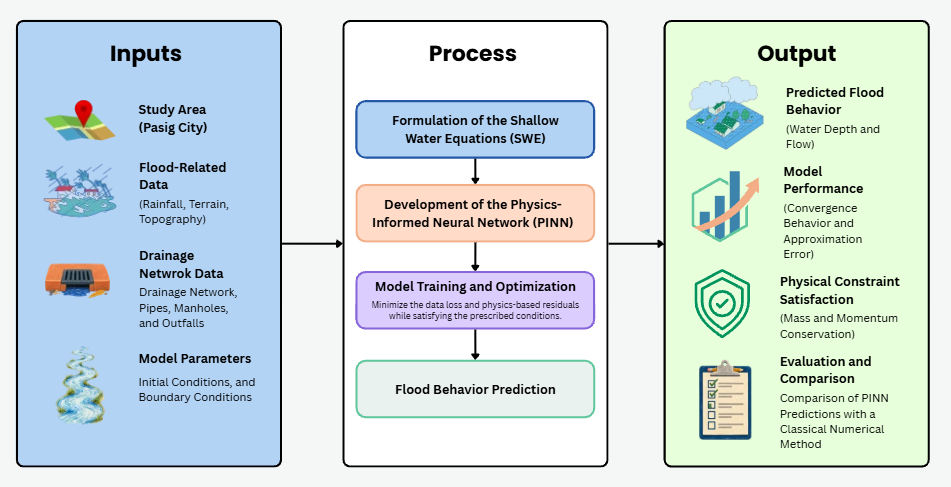
\includegraphics[width=0.95\textwidth]{assets/conceptual_framework.png}
    \caption{Conceptual Framework of the SWE-Based Physics-Informed Neural Network for Flood Modeling in Pasig City}
    \label{fig:conceptual_framework}
\end{figure}

The conceptual framework of the study follows an Input-Process-Output (IPO) model. It illustrates how the input data are processed through a Physics-Informed Neural Network incorporating the Shallow Water Equations to generate predictions of water depth, water flow, and flood behavior. 

\begin{enumerate}
    \item \textbf{Input Data:} The input data consist of rainfall data, terrain elevation, drainage network data, initial conditions, and boundary conditions for the selected study area in Pasig City. The drainage network data will provide information needed to incorporate the drainage rate into the governing equations. These inputs provide the environmental, spatial, and mathematical information required for the flood modeling process.

    \item \textbf{Process:} The input data will be processed using a SWE-based Physics-Informed Neural Network (PINN). The governing Shallow Water Equations, including the drainage rate as a representation of water removal through the drainage system, will be incorporated into the model's loss function as physical constraints. The network will undergo training and optimization by minimizing the data loss and the residuals of the governing equations while satisfying the specified initial and boundary conditions. Once trained, the model will be used to predict flood behavior across the selected study area.

    \item \textbf{Output:} The proposed model will generate predictions of water depth and horizontal water velocity, representing the flood behavior across the selected study area in Pasig City. The model will also be evaluated based on its convergence behavior, approximation error, and ability to satisfy the physical constraints represented by the conservation of mass and momentum.
\end{enumerate}

\section{Significance of the Study}

% Discuss the potential contributions of the study to flood modeling, disaster risk reduction, mathematical modeling, and the application of Physics-Informed Neural Networks. Identify the possible beneficiaries, such as local government units, disaster risk reduction offices, researchers, and future students.

This study aims to contribute to the development and evaluation of physics-informed computational approaches for flood modeling. By integrating the Shallow Water Equations into a neural network, the research will examine how physical constraints can be incorporated into flood prediction and how the resulting model performs compared with a classical numerical method.

\subsection{Local Government Units}

The findings of the study may provide useful information to local government units, particularly Pasig City, regarding the potential application of physics-informed neural networks in flood modeling. The predicted water depth and velocity may help improve the understanding of flood behavior in selected areas. However, the model is intended as a research-based computational approach and will not replace official flood forecasting systems.

\subsection{Disaster Risk Reduction and Management Offices}

The study may contribute to the development of computational approaches that can support flood assessment and disaster risk reduction. The results may provide additional insights into the movement and accumulation of water during flooding, which could be useful in understanding flood-prone areas.

\subsection{Researchers and the Academic Community}

This study may serve as a reference for researchers interested in mathematical modeling, numerical solutions of partial differential equations, and Physics-Informed Neural Networks. The comparison between the PINN and a classical numerical method may contribute to further investigations into the accuracy, convergence, and physical consistency of physics-informed models.

\subsection{Future Researchers and Students}

The study may serve as a foundation for future research involving PINNs and the Shallow Water Equations. Future researchers may extend the model by incorporating more detailed terrain data, additional hydrological variables, or more complex representations of urban drainage systems.

\section{Scope and Limitations}

% Define the coverage of the study, including the selected Philippine study area, the Shallow Water Equations, the input datasets, and the implementation of the SWE-based PINN.

% Discuss the limitations of the research, including data availability, spatial and temporal resolution, computational resources, and assumptions involved in the mathematical model.

This study will focus on the development and evaluation of a Shallow Water Equation-based Physics-Informed Neural Network for flood modeling in Pasig City, Philippines. The research will utilize the Shallow Water Equations as the governing mathematical model to represent the conservation of mass and momentum in water flow. The PINN will be developed to predict water depth and horizontal water velocity based on the available rainfall data, terrain elevation, initial conditions, and boundary conditions.

The study will evaluate the performance of the proposed PINN by comparing its numerical predictions with those obtained from a classical numerical method. The comparison will focus on convergence, approximation error, and physical consistency. Appropriate error metrics will be used to assess the differences between the two methods.

The scope of the study is limited to the selected study area within Pasig City and the available datasets. The accuracy of the model may be affected by the quality, completeness, and spatial and temporal resolution of the rainfall and terrain data. The availability of observed flood depth and water velocity measurements may also limit the extent of model validation.

Furthermore, the mathematical model will rely on the assumptions associated with the Shallow Water Equations, including the representation of water flow as a depth-averaged process. The study will not fully represent every physical factor that may influence urban flooding, such as highly detailed drainage network behavior, localized obstructions, or complex interactions between surface water and underground infrastructure. The model's computational performance may also depend on the available hardware and training configuration.

The study will primarily assess the PINN as a mathematical and computational approach to solving the Shallow Water Equations. Therefore, the findings will not necessarily establish the model's readiness for real-time operational flood forecasting or its applicability to all flood-prone areas in the Philippines.

\section{Definition of Terms}

% Provide the operational and conceptual definitions of important terms used throughout the study, including:

% Shallow Water Equations (SWE)
% Physics-Informed Neural Network (PINN)
% Flood Modeling
% Water Depth
% Horizontal Water Velocity
% Initial Conditions
% Boundary Conditions
% Approximation Error
% Convergence
% Conservation of Mass
% Conservation of Momentum

The following terms are defined conceptually and operationally to provide a clearer understanding of the concepts used in this study.

\begin{itemize}

    \item \textbf{Shallow Water Equations (SWE).}
    The Shallow Water Equations are a system of partial differential equations derived from the principles of conservation of mass and momentum. In this study, they serve as the governing mathematical model for representing water flow and flood behavior in Pasig City.

    \item \textbf{Physics-Informed Neural Network (PINN).}
    A Physics-Informed Neural Network is a neural network that incorporates governing physical equations into its training process through a loss function. In this study, the PINN will use the Shallow Water Equations as physical constraints to predict water depth and horizontal water velocity.

    \item \textbf{Flood Modeling.}
    Flood modeling refers to the mathematical and computational representation of flood behavior. In this study, it involves simulating water movement and estimating water depth and velocity within the selected study area.

    \item \textbf{Water Depth.}
    Water depth refers to the vertical distance between the ground surface and the water surface. In this study, it is one of the primary variables predicted by the SWE-based PINN.

    \item \textbf{Horizontal Water Velocity.}
    Horizontal water velocity refers to the rate and direction of water movement along the horizontal plane. In this study, it is represented by the velocity components in the $x$- and $y$-directions.

    \item \textbf{Initial Conditions.}
    Initial conditions specify the state of the modeled water system at the beginning of the simulation. In this study, they define the initial water depth and velocity values used in solving the Shallow Water Equations.

    \item \textbf{Boundary Conditions.}
    Boundary conditions describe the behavior of water flow along the boundaries of the computational domain. In this study, they define the constraints applied at the edges of the selected flood modeling area.

    \item \textbf{Approximation Error.}
    Approximation error refers to the difference between the solution produced by a computational method and a reference solution. In this study, it will be used to evaluate the accuracy of the PINN in comparison with the classical numerical method.

    \item \textbf{Convergence.}
    Convergence refers to the tendency of a numerical or computational solution to approach a stable or reference solution as the relevant approximation or training process progresses. In this study, it will be evaluated to examine the behavior of the PINN and the classical numerical method in solving the Shallow Water Equations.

    \item \textbf{Conservation of Mass.}
    Conservation of mass is the physical principle stating that mass is neither created nor destroyed within a system, although it may enter or leave through the system boundaries. In this study, it is represented by the continuity equation of the Shallow Water Equations.

    \item \textbf{Conservation of Momentum.}
    Conservation of momentum is the physical principle describing how the momentum of water changes due to forces such as gravity, friction, and flow interactions. In this study, it is represented by the momentum equations of the Shallow Water Equations.

\end{itemize}